\documentclass{scrartcl}
\usepackage[utf8]{inputenc}
\usepackage{graphicx}
%opening
\title{Preinforme 2 - Laboratorio de Electrónica}

\author{
	\footnotesize Hernández A., Alejandro\\
	\footnotesize \texttt{a.hernandez105@uniandes.edu.co}
	\and
	\footnotesize Prada G., Jesús David\\
	\footnotesize \texttt{jd.prada1760@uniandes.edu.co}
       }
\date{\vspace{-5ex}}
%\date{}

\setlength{\parindent}{0pt}
\renewcommand{\indent}{\hspace*{\tindent}}

\begin{document}

\maketitle

\begin{abstract}
\small
En esta práctica de laboratorio se pretende aprender el funcionamiento experimental de elementos electrónicos tales como diodos, transistores y LEDs con el fin de reproducir mediante el uso de dichos elemementos el funcionamiento de compurtas lógicas y switches.
\end{abstract}

\section{Diodos}

Un diodo es un componente electrónico de dos terminales conconductancia asimétrica, esto es, permite el paso de corriente con resistencia nula en una dirección mientras que impide totalmente el paso de la misma en dirección opuesta.\\

Los diversos tipos de diodos que existen se muestran en la figura \ref{fig: diodos1}.

\begin{figure}[h!]
	\centering
	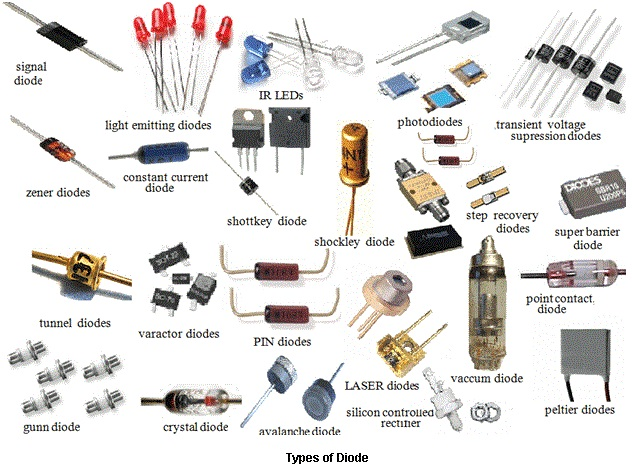
\includegraphics[width=0.85\textwidth]{diodos1}
	\caption{Tipos de diodos.}
	\label{fig: diodos1}
\end{figure}

\begin{figure}[h!]
	\centering
	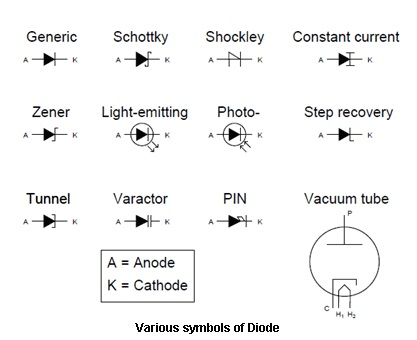
\includegraphics[width=0.6\textwidth]{diodos2}
	\caption{Tipos de diodos.}
	\label{fig: diodos2}
\end{figure}

Las características de los tipos de diodos más frecuentemente usados se describen a continuación:

\begin{itemize}
	\item \textbf{Diodos termoiónicos:} También llamados diodos de vacío, este tipo de diodos consisten básicamente de un arreglo de dos electrodos empacados al vacío dentro de una tubo de vidrio. Uno de los electrodos es un cátodo calentado por un filamento, el otro electrodo es una lámina (ánodo) y el voltaje alternante a ser rectificado es aplicado entre el cátodo y la lámina concéntrica. Cuando el cátodo es calentado, emite electrones al vacío por medio de un proceso llamado emisión termoiónica. Si la lámina tiene un voltaje positivo con respecto al cátodo, dicha lámina atrae electrostáticamente a los electrones, creando una corriente del cátodo a la lámina. En caso contrario, no se genera niguna corriente puesto que la lámina no atrae a los electrones.
	
	\item \textbf{Diodos semiconductores:} También denominados diodos de juntura, estos diodos se componen de un cristal semiconductor (como silicio o germanio) dopado con impurezas con el fin de generar dos regiones, a saber, una región que contenga portadores de carga negativa (electrones), llamada semiconductor de tipo n, y una región que contenga portadores de carga positiva (huecos), llamada seminconductor tipo p. Cuando las dos zonas se unen a través de las terminales del diodo (juntura p-n) un flujo momentáneo de electrones ocurre de la región n a la región p, dando como resultado una tercera zona, llamada de agotamiento, donde no hay portadores de carga. En este caso, el cristal permite el flujo de electrones de la zona n a la zona p, pero no en dirección opuesta.
	
	\item \textbf{Diodos Schottky:} Caso particular de diodos semiconductores, formados por una juntura metal-seminconductor en vez de una juntura p-n, causando de esta manera una reducción en la capacitancia y un incremento en la velocidad de cambio del diodo.
	
	\item \textbf{Diodos emisores de luz (LEDs):} Si un diodo es formado a partir de un semiconductor de band gap directo (como el arseniuro de galio), los portadores de carga que cruzan la juntura p-n emiten fotones al recombinarse con los portadores de carga del otro lado de la juntura. Dependiendo del material, las longitudes de onda producidas van desde el infrarrojo hasta el untravioleta. La diferencia de potencial a través de estos diodos depende de la longitud de onda emitida, siendo $2.1\ V$ para el rojo, o $4\ V$ para el violeta. 

	\item \textbf{Diodos túnel:} Este tipo de diodos poseen una región de operación en la que muestran una resistencia negativa generada por el tunelamiento cuántico de electrones entre las terminales del diodo, permitiendo, por ejemplo, la amplificación de señales. Debido a la alta concentración de portadores de carga, los diodos túnel	son muy rápidos, pueden ser usados a temperaturas del orden de $mK$, con campos magnéticos grandes y en ambientes de alta radiación. Típicamente son usados en naves espaciales.

\end{itemize}

Existen muchos otros tipos de diodos aparte de los mencionados anteriormente, tales como diodos láser, diodos térmicos, diodos Zener, entre otros, pero solo quisimos referirnos a los más usados en situaciones comunes (no muy avanzadas) de laboratorio.

OJO - FALTA PONER LO DEL KIT	

\section{Rectificadores de onda completa con diodos}

.
\\



\section{Mediciones con voltímetro}

Para medir voltajes se debe de conectar el multímetro a los extremos de los componentes que se desean medir. La siguiente imagen muestra cómo hacerlo.
\\ 


Análogamente, para medir corrientes el multímetro debe ubicarse en el paso de la corriente que se desea medir, tal como lo ilustra la siguiente figura.
\\ 


\section{Osciloscopio}
Un osciloscopio es un aparato que sirve para medir y visualizar las señales de salida de un circuito. Su interfaz gráfica permite el análisis cualitativo y facilita la toma de diversos datos en la dinámica del circuito estudiado. El osciloscopio que usaremos es de marca Tektronix, de la serie TDS 210. En la siguiente figura se puede apreciar el panel frontal del osciloscopio, el cual se compone de una pantalla y una serie de botones, perillas y entradas cuya función explicaremos más adelante.\\


Los comandos del osciloscopio están organizados por funciones. Los botones cercanos a la pantalla permiten navegar por diversas opciones e interactuar con la interfaz gráfica del osciloscopio. Los botones de la parte superior permiten seleccionar diferentes menús y controlar la señal de entrada. Por otra parte, hay grupos de comandos que permiten mover y modificar los cursores en la pantalla. Estos cursores se usan principalmente para seleccionar un punto específico de la señal en la pantalla. Además de estos, hay un grupo de comandos que sirven para modificar el trigger, el cual permite controlar el muestreo de las señales periódicas. En la siguiente figura se puede apreciar el grupo de controladores verticales del cursor.\\


Donde los comandos tienen las siguientes funciones:
\begin{itemize}
	\item \textbf{Position:} Controla la posición vertical del cursor o del canal. 
	\item \textbf{CH Menu:} Muestra el menú de entrada de canal y permite mostrar o quitar la señal de dicho canal.
	\item \textbf{Math Menu:} Muestra el menu de operaciones matemáticas para las señales.
	\item \textbf{Volts/Div:} Permite modificar las escalas en las que se muestran la señal en el eje vertical.

\end{itemize}

En la siguiente figura se muestra por su parte, el grupo de controladores horizontales.


Donde los comandos tienen las siguientes funciones:
\begin{itemize}
	\item \textbf{Position:} Controla la posición horizontal de todos los canales.
	\item \textbf{Horizontal Menu:} Muestra el menu de medida horizontal.
	\item \textbf{Sec/Div:} Permite modificar las escalas en las que se muestran la señal en el eje horizontal.
\end{itemize}

Los controladores de trigger se muestran en la siguiente figura 10. Allí los comandos tienen las siguientes funciones:

\begin{itemize}
	\item \textbf{Level-Holdoff:} En el modo Level, modifica la amplitud que tiene que cruzar la señal para causar una adquisición. En modo Holdoff, selecciona el tiempo antes de que otro trigger pueda ser aceptado.
	\item \textbf{Trigger Menu:} Muestra el menu de trigger.
	\item \textbf{Set Level to 50\%:} Modifica el nivel del trigger al 50\% del nivel de la señal.
	\item \textbf{Force Trigger:} Empieza la adquisición sin importar si la amplitud de la señal supera el trigger.
	\item \textbf{Trigger View:} Muestra el trigger.
\end{itemize}

En la figura 11 se pueden ver los comandos de control general. \\


Estos tienen las siguientes funciones:

\begin{itemize}
	\item \textbf{Save/Recall:} Muestra el menú para salvar y cargar señales.
	\item \textbf{Measure:} Muestra el menú de medidas.
	\item \textbf{Acquire:} Muestra el menú de adquisición de la señal.
	\item \textbf{Cursor:} Muestra el menú de cursores donde se permite controlar qué cursor se mueve con los paneles de comandos horizontales y verticales.
	\item \textbf{Utility:} Muestra el menú de utilidades.
	\item \textbf{Autoset:} Selecciona automáticamente los parámetros para mostrar una señal útil. (No siempre funciona)
	\item \textbf{Hardcopy:} Se usa para imprimir. Necesita una impresora especial conectada al dispositivo.
	\item \textbf{Run/Stop:} Empieza o termina el muestreo.\\
\\
Entre otras opciones la función Measure permite hacer diversas medidas de la señal analizada. En el osciloscopio con el que trabajaremos podremos medir el voltaje rms en un ciclo, el voltaje medio, el voltaje pico-pico, el periodo y la frecuencia de la señal analizada.

\end{itemize}


\section{Generador de señales}
Un generador de señales es una fuente de potencial que permite generar voltajes de forma sinusoidal, cuadrada o triangular. Este dispositivo permite también modificar la frecuencia y la amplitud de estas señales. En el laboratorio utilizaremos un generador marca Tektronix de la serie CFG253. En la siguiente figura se puede ver una fotografía de la parte frontal de dos de estos generadores.\\

En la figura 13 se ve un diagrama claro de los comandos de este dispositivo. Aquí las funciones son las siguientes:

\begin{itemize}
	\item \textbf{1:} Muestra si el dispositivo está encendido o apagado.
	\item \textbf{2:} Determina la amplitud de la señal que sale por el cable principal (main).
	\item \textbf{3:} Sirve para controlar la aplitud DC de la señal y su polaridad.
	\item \textbf{4:} Controla la simetría vertical de la señal generada.
	\item \textbf{5:} Determina el rango en que se va a modificar la frecuencia de la señal que sale por el cable principal.
	\item \textbf{6:} Selecciona la forma de la onda de salida: sinusoidal, cuadrada o triangular.
	\item \textbf{7:} Modifica la frecuencia en el rango determindo por (5).
	\item \textbf{8:} Ajusta la amplitud de barrido de la señal.
	\item \textbf{9:} Ajusta la frecuencia del generador de barrido interno.
	\item \textbf{10:} Activa las opciones (8) y (9).
	\item \textbf{11:} Divide la frecuencia de la señal de salida por 10 y permite ajustar la simetría de la señal con (4).
	\item \textbf{12:} Permite variar el rango en el que se controla la amplitud del voltaje pico-pico de la señal.




\end{itemize}
	
	
\end{document}








